\documentclass{article}
\usepackage[utf8]{inputenc}
\usepackage{amsmath, amssymb, amsthm}
\usepackage{graphicx}
\usepackage{geometry}
\usepackage{listings}
\usepackage{xcolor}

\geometry{a4paper, margin=1in}

% Code snippet formatting
\definecolor{codegreen}{rgb}{0,0.6,0}
\definecolor{codegray}{rgb}{0.5,0.5,0.5}
\definecolor{codepurple}{rgb}{0.58,0,0.82}
\definecolor{backcolour}{rgb}{0.95,0.95,0.92}

\lstdefinestyle{mystyle}{
    backgroundcolor=\color{backcolour},   
    commentstyle=\color{codegreen},
    keywordstyle=\color{magenta},
    numberstyle=\tiny\color{codegray},
    stringstyle=\color{codepurple},
    basicstyle=\ttfamily\small,
    breakatwhitespace=false,         
    breaklines=true,                 
    captionpos=b,                    
    keepspaces=true,                 
    showspaces=false,                
    showstringspaces=false,
    showtabs=false,                  
    tabsize=4
}
\lstset{style=mystyle}

\title{MIT 6.s184 / 6.s978 Deep Generative Models \\ Problem Set 1 Report}
\author{Your Name} % 请在这里填入你的名字
\date{\today}

\begin{document}

\maketitle

\section*{Problem 1: Auto-Encoder on MNIST}
\subsection*{(a) AE Implementation}
The encoder and decoder for the Auto-Encoder are implemented as follows:
\begin{lstlisting}[language=Python]
# --- 1. Encoder ---
encoder_layers = [] 
in_dim = input_dim 
for out_dim in hidden_dims:
    encoder_layers.append(torch.nn.Linear(in_dim, out_dim))
    if out_dim != hidden_dims[-1]: 
        encoder_layers.append(torch.nn.ReLU())
    in_dim = out_dim 
self.encoder = torch.nn.Sequential(*encoder_layers)

# --- 2. Decoder ---
decoder_layers = []
in_dim = hidden_dims[-1]
for out_dim in reversed(hidden_dims[:-1]):
    decoder_layers.append(torch.nn.Linear(in_dim, out_dim))
    decoder_layers.append(torch.nn.ReLU())
    in_dim = out_dim
decoder_layers.append(torch.nn.Linear(in_dim, input_dim))
decoder_layers.append(torch.nn.Sigmoid())
self.decoder = torch.nn.Sequential(*decoder_layers)
\end{lstlisting}

\subsection*{(b) AE Training and Evaluation}
% 提示：请将你在 Jupyter 中跑出的图片保存到根目录，并替换这里的文件名。也可以直接截图贴在 Word 中再导出 PDF。
\begin{figure}[h]
    \centering
    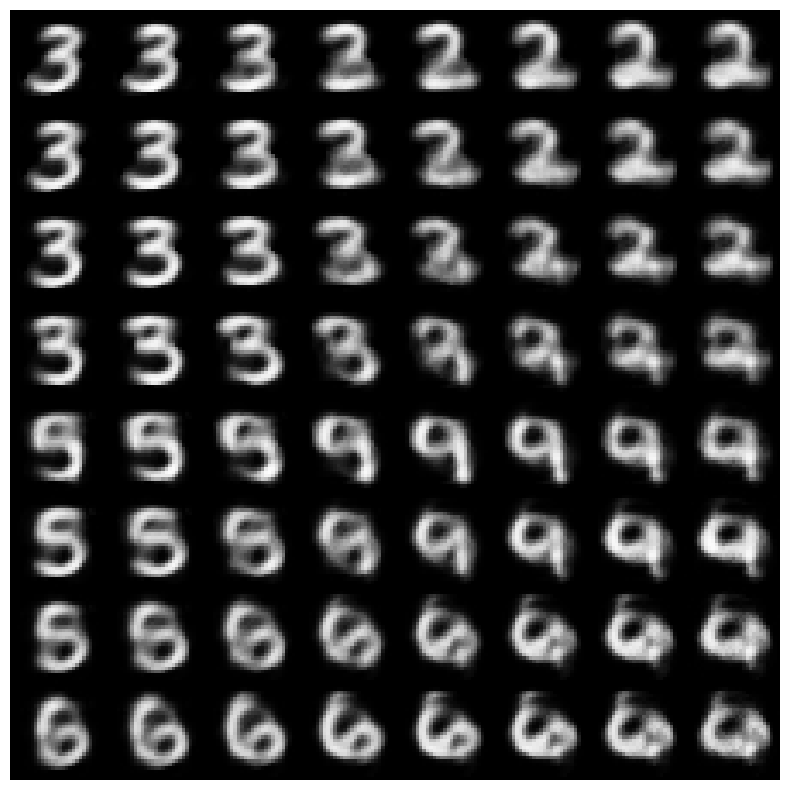
\includegraphics[width=0.8\textwidth]{ae_results.png}
    \caption{AE Reconstruction and Interpolation Results on MNIST.}
\end{figure}

\section*{Problem 2: Variational Auto-Encoder on MNIST: SGVB}
\subsection*{(a) Proof of the ELBO}
We start from the marginal log-likelihood $\log p(x)$. By introducing a variational distribution $q(z|x)$ and applying Jensen's Inequality (since the logarithmic function is concave), we derive the ELBO:
\begin{align*}
\log p(x) &= \log \int p(x, z) \, dz \\
&= \log \int q(z|x) \frac{p(x, z)}{q(z|x)} \, dz \\
&= \log \mathbb{E}_{q(z|x)} \left[ \frac{p(x, z)}{q(z|x)} \right] \\
&\geq \mathbb{E}_{q(z|x)} \left[ \log \frac{p(x, z)}{q(z|x)} \right] \quad \text{(by Jensen's Inequality)}
\end{align*}
Thus, the Evidence Lower Bound (ELBO) is $\mathbb{E}_{q(z|x)} \left[ \log \frac{p(x, z)}{q(z|x)} \right]$.

\subsection*{(b) VAE Encoder and Decoder}
\begin{lstlisting}[language=Python]
# --- 1. Encoder ---
encoder_layers = []
in_dim = input_dim
for i, out_dim in enumerate(hidden_dims):
    encoder_layers.append(torch.nn.Linear(in_dim, out_dim))
    if i < len(hidden_dims) - 1:
        encoder_layers.append(torch.nn.ReLU())
    in_dim = out_dim
self.encoder = torch.nn.Sequential(*encoder_layers)

# --- 2. Decoder ---
decoder_layers = []
in_dim = self.z_size
for out_dim in reversed(hidden_dims[:-1]):
    decoder_layers.append(torch.nn.Linear(in_dim, out_dim))
    decoder_layers.append(torch.nn.ReLU())
    in_dim = out_dim
    
final_out_dim = input_dim if decode_dim == -1 else decode_dim
decoder_layers.append(torch.nn.Linear(in_dim, final_out_dim))

if use_sigmoid:
    decoder_layers.append(torch.nn.Sigmoid()) 

self.decoder = torch.nn.Sequential(*decoder_layers)
\end{lstlisting}

\subsection*{(c) Reparameterization Trick}
\begin{lstlisting}[language=Python]
def reparameterize(self, mean, logvar, n_samples_per_z=1):
    std = torch.exp(0.5 * logvar)
    eps = torch.randn_like(std) 
    z = eps * std + mean 
    return z
\end{lstlisting}

\subsection*{(d) SGVB log\_normal\_pdf}
\begin{lstlisting}[language=Python]
def log_normal_pdf(sample, mean, logvar, raxis=1):
    log_p = -0.5 * (log2pi + logvar + ((sample - mean) ** 2) / torch.exp(logvar))
    return torch.sum(log_p, dim=raxis)
\end{lstlisting}

\section*{Problem 3: VAE on MNIST: Analytical KL Divergence}
\subsection*{(a) Proof of ELBO Decomposition}
Given $p(z) = \mathcal{N}(z; 0, I)$ and $q(z|x) = \mathcal{N}(z; \mu(x), \text{diag}(\sigma^2(x)))$:
\begin{align*}
\text{ELBO} &= \mathbb{E}_{q(z|x)} \left[ \log \frac{p(x, z)}{q(z|x)} \right] \\
&= \mathbb{E}_{q(z|x)} [ \log p(x|z) + \log p(z) - \log q(z|x) ] \\
&= \mathbb{E}_{q(z|x)} [ \log p(x|z) ] - D_{KL}(q(z|x) \parallel p(z))
\end{align*}
The KL divergence between a multivariate Gaussian with diagonal covariance and a standard normal distribution decomposes dimension-wise. For each dimension $d$:
\begin{align*}
-D_{KL}(q(z_d|x) \parallel p(z_d)) &= \int q(z_d|x) \log \frac{p(z_d)}{q(z_d|x)} dz_d \\
&= \mathbb{E}_{q} \left[ -\frac{1}{2}\log(2\pi) - \frac{1}{2}z_d^2 - \left(-\frac{1}{2}\log(2\pi\sigma_d^2) - \frac{(z_d - \mu_d)^2}{2\sigma_d^2}\right) \right] \\
&= \mathbb{E}_{q} \left[ \frac{1}{2}\log(\sigma_d^2) - \frac{1}{2}z_d^2 + \frac{(z_d - \mu_d)^2}{2\sigma_d^2} \right]
\end{align*}
Since $\mathbb{E}_{q}[z_d^2] = \mu_d^2 + \sigma_d^2$ and $\mathbb{E}_{q}[(z_d - \mu_d)^2] = \sigma_d^2$:
\begin{align*}
-D_{KL}(q(z_d|x) \parallel p(z_d)) &= \frac{1}{2}\log(\sigma_d^2) - \frac{1}{2}(\mu_d^2 + \sigma_d^2) + \frac{1}{2} \\
&= \frac{1}{2} \left(1 + \log(\sigma_d^2) - \mu_d^2 - \sigma_d^2\right)
\end{align*}
Summing over all dimensions $d$ gives:
$$ -D_{KL}(q(z|x) \parallel p(z)) = \frac{1}{2}\sum_d \left(1 + \log(\sigma_d^2) - \mu_d^2 - \sigma_d^2\right) $$
This yields the required analytical decomposition.

\subsection*{(b) SGVB vs Analytical KL Curves}
% 提示：保存 jupyter 运行出的对比曲线图，去掉注释并将图片引用进来
\begin{figure}[h]
    \centering
    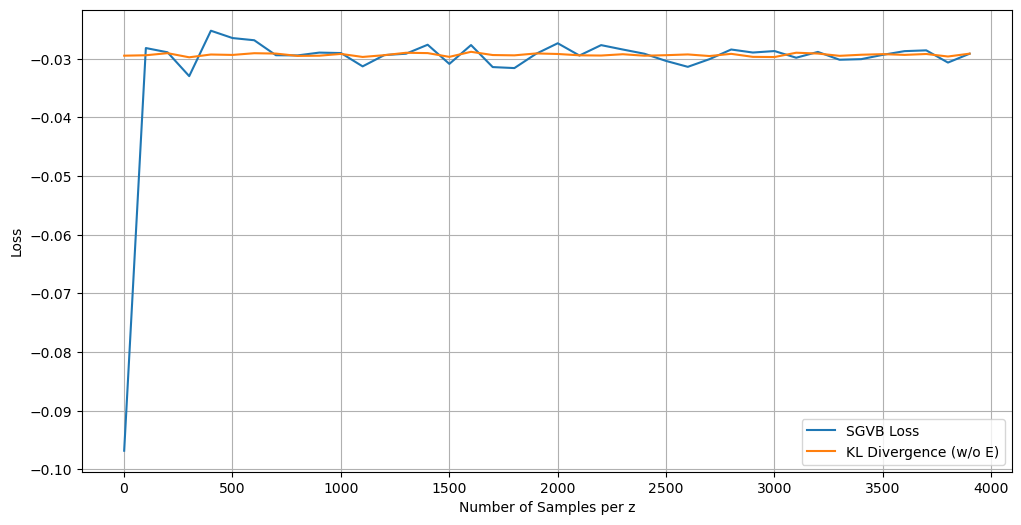
\includegraphics[width=0.6\textwidth]{kl_vs_sgvb.png}
    \caption{SGVB Estimator vs Analytical KL Divergence.}
\end{figure}

\subsection*{(c) Training VAEs with both losses}
\begin{figure}[h]
    \centering
    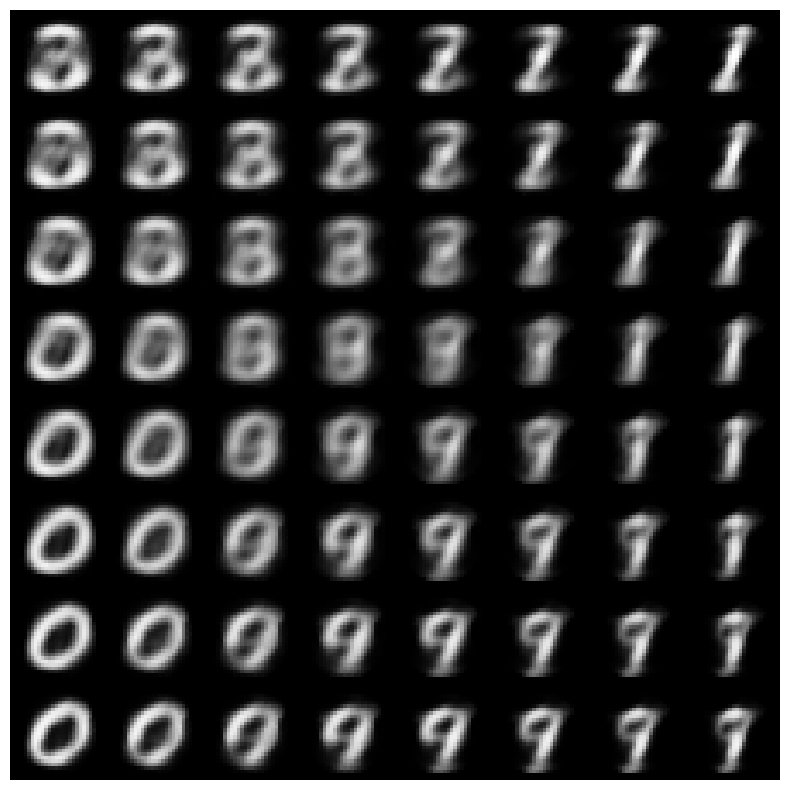
\includegraphics[width=0.45\textwidth]{vae_sgvb.png}
    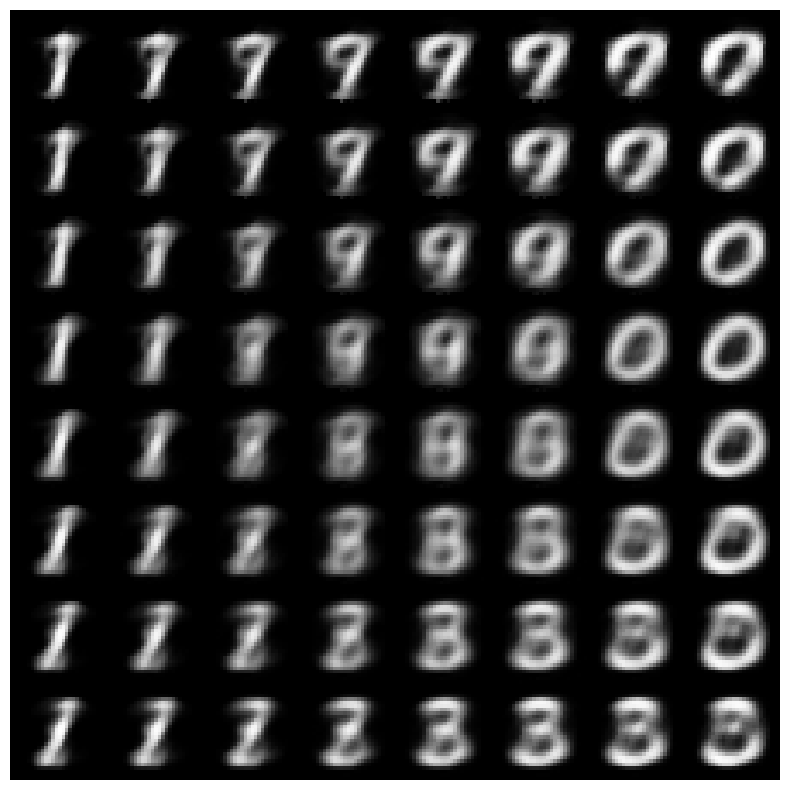
\includegraphics[width=0.45\textwidth]{vae_kl.png}
    \caption{VAE Results using SGVB (Left) and Analytical KL (Right).}
\end{figure}


\section*{Problem 4: VAE on Torus Point Cloud}
\subsection*{(a) Reconstruction Results}
\begin{figure}[h]
    \centering
    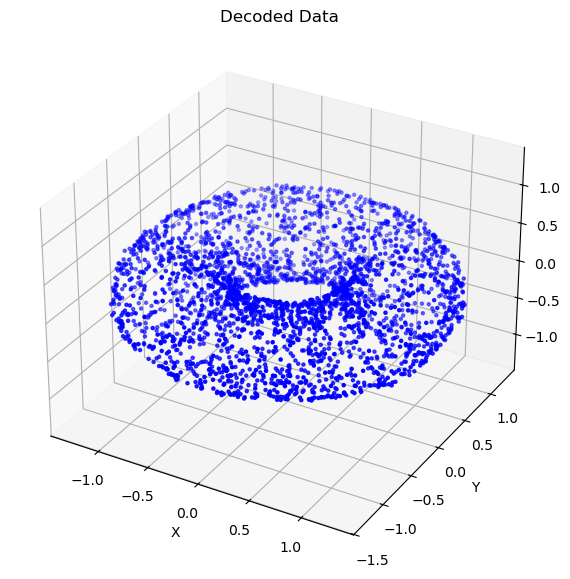
\includegraphics[width=0.6\textwidth]{torus_recon.png}
    \caption{Torus Point Cloud Reconstruction.}
\end{figure}

\subsection*{(b) Linear Interpolation}
\begin{figure}[h]
    \centering
    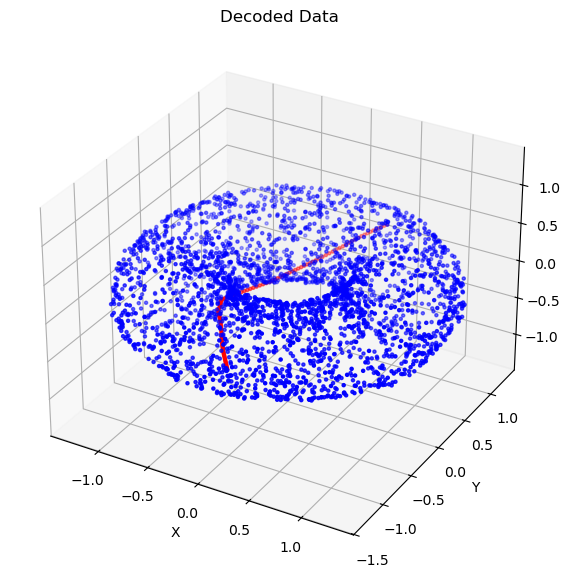
\includegraphics[width=0.6\textwidth]{torus_interp.png}
    \caption{Linear Interpolation Output mapped to Torus.}
\end{figure}

\subsection*{(c) Architecture Modification for Intrinsics (Optional)}
To better capture the intrinsic toroidal structure of the data, the architecture utilizes a \textbf{Positional Encoding} layer before the VAE encoder. This transforms the original 3D coordinates $(x,y,z)$ into a high-dimensional feature space using sine and cosine functions across multiple frequency bands. 

By directly initializing the VAE with these multi-frequency inputs inside the \texttt{PointVAE} module (with \texttt{use\_sigmoid=False}), the neural network overcomes spectral bias. This effectively enforces the decoded interpolation trajectory to adhere to the curved geometry of the Torus, correctly mapping linear traversals in the latent space to geodesic paths along the surface of the 3D object.

\end{document}
